\documentclass{exam}
\usepackage{../../mypackages}
\usepackage{../../macros}

\setlength{\parindent}{0pt}

\title{Interro N°1 - Masse volumique + Atome}
\author{N. Bancel}
\date{3 Octobre 2024}

\begin{document}

\textbf{Collège Lycée Suger}
\hfill
\textbf{Physique-Chimie} \\

\textbf{Année 2024-2025}
\hfill
\textbf{3ème Cambridge International} \par

{\let\newpage\relax\maketitle}
%\maketitle

\begin{center}
  \textbf{\textcolor{red}{La calculatrice n'est pas autorisée}}
  \end{center}

\section*{Masse volumique}

\begin{questions}
  \question[0.5] Définir rapidement ce que signifie "l'unité légale dans le système international".
  \question[1] Quelle est l'expression de la masse volumique d'un matériau ? Préciser les unités légales dans le système international de chaque variable
  \question[1] Formules déduites 
  \begin{itemize}
    \item Si l'on dispose de la valeur du volume, et de la masse volumique d'un corps, quelle expression permet d'en déduire la masse ?
    \item Si l'on dispose de la valeur de la masse, et de la masse volumique d'un corps, quelle expression permet d'en déduire le volume ?
  \end{itemize}
  \question[2] La masse volumique du sable est de \SI{1850}{kg/m^3} en moyenne. Pour un chantier, une entreprise de maçonnerie a besoin de \SI{50}{tonnes} de sable.
  \begin{itemize}
    \item \textcolor{blue}{Indication : $\frac{50}{18.5} \approx 2.702$ et $\frac{60.2}{21} \approx 2.866$}
    \item Peut-elle les transporter dans un camion benne de \SI{21}{m^3} ? Pourquoi ?
    \item Si l'on suppose que le 1er camion a été intégralement rempli de sable, quel est le \text{\%} de remplissage du 2ème camion ?
\end{itemize}

\question[2] Effectuer les conversions suivantes : 
  \begin{itemize}
    \item \SI{1}{kg} = .... \SI{}{g}
    \item \SI{1}{L} = .... \SI{}{cL} = .... \SI{}{mL}
    \item \SI{1}{m^3} = .... \SI{}{dm^3} = .... \SI{}{L}
    \item \SI{1}{kg/m^3} = .... \SI{}{g/L}
\end{itemize}

\end{questions}

\section*{L'atome}

\begin{questions}
  \question[1] A partir du schéma ci-dessous, remplir les légendes (1), (2), (3). Quel est le nom plus global pour les particules (2) et (3) ?

  \begin{figure}[H]
    \centering
    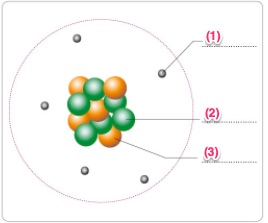
\includegraphics[width=0.6\linewidth]{interro1_01.jpg}
    \caption{Structure de l'atome}
  \end{figure}

  \question[1] Un atome est souvent symbolisé par le schéma ci-dessous. Que signifient $A$, $X$, et $Z$ ?

  \begin{figure}[H]
    \centering
    
\includegraphics[width=0.3\linewidth]{interro1_02.jpg}
    \caption{Symbole de l'atome}
  \end{figure}

  \question[1] Comment détermine-t-on le nombre de neutrons dans un atome ?
  \question[0.5] On dit que l'atome est électriquement neutre : pourquoi ?

  
\end{questions}

\end{document}
